\hypertarget{pmlsc-large-scale-condensation}{%
\subsection{pmlsc: Large Scale
Condensation}\label{pmlsc-large-scale-condensation}}

The SUBROUTINE:{[}PDF2CLD{]} and SUBROUTINE:{[}CLD2PDF{]} are written in
pmlsc.F file. These are called in padmn.F, pcumc.F, pshcn.F, pcldphys.F
and pvdfm.F files.

\hypertarget{physical-basis-for-statistical-pdf-scheme}{%
\subsubsection{Physical basis for statistical PDF
scheme}\label{physical-basis-for-statistical-pdf-scheme}}

General Circulation Models (GCMs) typically adopt fractional cloud cover
(the volume of cloudy air per total air volume in a grid box) assumption
to realistically represent clouds because of their coarse horizontal
resolution (\(O(100km)\)). Statistical cloud schemes assume a
subgrid‐scale probability density function (PDF) of humidity within the
grid. Integration of the specific PDFs will give the cloud fraction and
the amount of water condensate consistently.

By means of the ``fast condensation'' assumption, the cloud water amount
in a local area in the grid is

\begin{eqnarray}
q_{c}=\left(q_{t}-q_{s}\right) \delta\left(q_{t}-q_{s}\right)
\label{hpc.1}
\end{eqnarray}

where \(q_s\) denotes the saturation mixing ratio and \(q_c\) does the
cloud water ratio. \(q_t\) is sum of water vapor and cloud water mixing
ratio. \(\delta(x)\) denotes the Heviside function of x.

The majority of statistical cloud schemes use the so-called
``s-distribution'' following Sommeria and Deardorff (1977). A single
variable \(s\), which considers the subgrid-scale perturbations of
liquid temperature \(T_l\) and total water mixing ratio \(q_t\), is
employed. \(s\) is defined as

\begin{eqnarray}
s=a_{L}\left(q_{t}-\alpha_{L} T_{l}\right)
\end{eqnarray}

where

\begin{eqnarray}
a_{L}=1 /\left(1+L \alpha_{L} / c_{p}\right), \alpha_{L}=\partial q_{s} /\left.\partial T\right|_{T=\bar{T_l}}.
\end{eqnarray}

For any choice of the PDF of \(s\), denoted as \(G(s)\), the grid-mean
cloud fraction, \(C\), and cloud water content, \(q_c\), are obtained by
integrating \(G(s)\) and \((Qc + s)G(s)\),

\begin{eqnarray}
C=\int_{-Q_{c}}^{\infty}G(s)ds
\end{eqnarray}

\begin{eqnarray}
\bar{q}_{c}=\int_{-Q_{c}}^{\infty}\left(Q_{c}+s\right)G(s)ds,
\end{eqnarray}

where \(Qc\) denotes the grid-scale saturation deficit defined as \begin{eqnarray}
Q_{c} \equiv a_{L}\left\{\bar{q}_{t}-q_{s}\left(\bar{T}_{l}, \bar{p}\right)\right\}.
\end{eqnarray}

\hypertarget{hybrid-prognostic-cloud-hpc-scheme}{%
\subsubsection{Hybrid Prognostic Cloud (HPC)
scheme}\label{hybrid-prognostic-cloud-hpc-scheme}}

The statistical scheme implemented in MIROC6 is called Hybrid Prognostic
Cloud (HPC) scheme (Watanabe et al.~2009). The HPC scheme proposes two
types of shape for the PDF \(G(s)\), Double-uniform PDF and
Skewed-triangular PDF. Here we focus on Skewed-triangular scheme because
MIROC6 adoptes the shape. The physical basics of the scheme are in
common with Double-uniform PDF.

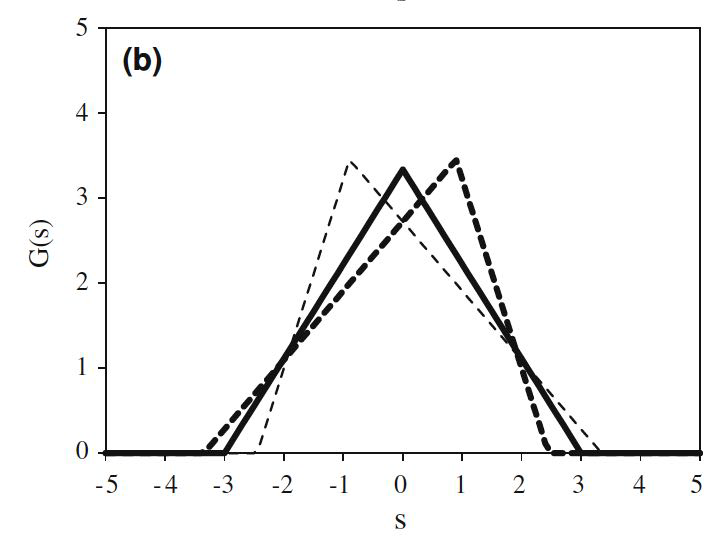
\includegraphics{Hotta_pmlsc_PDF.png}

Example of the basis PDF for HPC: skewed-triangular functions. Copied
from Fig.1 in Watanabe et al.~2009.

The scheme preicts variance (\(V\)) and skewness (\(S\)) of the PDF.
\(V\), \(S\), the second moment \(\mu_2\), and the third moment
\(\mu_3\) are defined as follows.

\begin{eqnarray}
\mu_{2} \equiv V=\int_{-\infty}^{\infty} s^{2} G(s) ds
\end{eqnarray}

\begin{eqnarray}
\mu_{3} \equiv \mu_{2}^{3 / 2} S=\int_{-\infty}^{\infty} s^{3} G(s) d s
\end{eqnarray}

\(V\) and \(S\) are affected by cumulus convection, cloud microphysics,
turbulent mixing, and advection.

The integrals to obtain \(C\) and \(q_c\) is symbolically expressed as

\begin{eqnarray}
C=I_{C}\left(\bar{p}, \bar{T}_{l}, \bar{q}_{t}, \mathcal{V}, \mathcal{S}\right)
\label{W09-1}
\end{eqnarray}

\begin{eqnarray}
\bar{q}_{c}=I_{q}\left(\bar{p}, \bar{T}_{l}, \bar{q}_{t}, \mathcal{V}, \mathcal{S}\right)
\label{W09-2}
\end{eqnarray}

where \(\bar{p}\) denotes the pressure. The overbars denote the
grid-mean quantity.

If the PDF is not too complicated, (1, 2) can be analytically solved for
\(V\) and \(S\) by defining integrand functions \({\tilde{I}}\) as

\begin{eqnarray}
\mathcal{V}=\tilde{I}_{\mathcal{V}} \left(\bar{p}, \bar{T}_{l}, \bar{{q}}_{v}, \bar{q}_{c}, C\right)
\label{W09-4}
\end{eqnarray}

\begin{eqnarray}
\mathcal{S}=\tilde{I}_{\mathcal{S}} \left(\bar{p}, \bar{T}_{l}, \bar{{q}}_{v}, \bar{q}_{c}, C\right)
\label{W09-5}
\end{eqnarray}

The relationship between (1, 2) and (4, 5) is quasireversible. The
double-uniform function and skewed-triangular function PDFs are selected
for \(G(s)\) because of their feasibility in analytically nalderiving
\({\tilde{I}}\).

\hypertarget{pdf-change-through-processes}{%
\subsubsection{PDF change through
processes}\label{pdf-change-through-processes}}

The HPC cloud scheme is composed using prognostic equations for four
variables determining \(I\), namely, \(T_l\), \(q_t\), \(V\), and \(S\).
The prognostic variables can be \(T_l\), \(q_t\), \(C\), and \(q_c\)
that determine \(\tilde {I}\).

Prognostic equations for the PDF variance and skewness are expressed as

\begin{eqnarray}
\frac{D \mathcal{V}}{D t}=\left.\frac{\Delta \mathcal{V}}{\Delta t}\right|_{\mathrm{conv.}}+\left.\frac{\Delta \mathcal{V}}{\Delta t}\right|_{\mathrm{micro.}}+\left.\frac{\Delta \mathcal{V}}{\Delta t}
\right|_{\mathrm{turb.}}+\left.\frac{\Delta \mathcal{V}}{\Delta t}
\right|_{\mathrm{others}}-\varepsilon \mathcal{V}
\end{eqnarray}

\begin{eqnarray}
\frac{D \mathcal{S}}{D t}=\left.\frac{\Delta \mathcal{S}}{\Delta t}\right|_{\mathrm{conv.}}+\left.\frac{\Delta \mathcal{S}}{\Delta t}\right|_{\text {micro.}}+\left.\frac{\Delta \mathcal{S}}{\Delta t}
\right|_{\mathrm{turb.}}+\left.\frac{\Delta \mathcal{S}}{\Delta t}\right|_{\text {others}}-\varepsilon_{\mathcal{S}}
\end{eqnarray}

where subscripts `conv.', `micro.' and `turb.' indicate cumulus
convection, cloud microphysics and turbulent mixing processes, which all
affect the PDF shape. The last terms represent dissipation due to
subgrid-scale horizontal motions. The specific formulations for each
term are described below.

The HPC scheme is referred to as and \(G(s)\) is updated every after the
process that affects cloud water PDF. \(G(s)\) is thus modified several
times within a single time step.

\hypertarget{cumulus-convection}{%
\paragraph{Cumulus convection}\label{cumulus-convection}}

The total effect of cumulus convection to the PDF moments is written as

\begin{eqnarray}
\left.\frac{\Delta \mathcal{V}}{\Delta t}\right|_{\mathrm{conv} .}=M_{c} \frac{\partial \mathcal{V}}{\partial z}+\frac{\Delta \tilde{I}_{\mathcal{V}}}{\Delta t}
\label{W09-14}
\end{eqnarray}

\begin{eqnarray}
\left.\frac{\Delta \mathcal{S}}{\Delta t}\right|_{\mathrm{conv} .}=M_{c} \frac{\partial \mathcal{S}}{\partial z}+\frac{\Delta \tilde{I}_{\mathcal{S}}}{\Delta t}
\label{W09-15}
\end{eqnarray}

\(M_c\) is the cumulus mass-flux including updraft in the convection
tower and downdraft in the environment. The vertical transport of the
PDF moments is represented by the first terms on the right side hand of
(14, 15).

Cumulus convections modify the grid-mean \(T_l\), \(q_t\), and \(q_c\)
by upward transportation of grid-mean moist static energy, \(q_v\), and
\(q_c\). Detrainment also affects these variables. The detrainment of
the cloudy air mass is considered, as in Bushell et al.~(2003),

\begin{eqnarray}
\left.\frac{\partial C}{\partial t}\right|_{\mathrm{conv} .}=D(1-C)
\end{eqnarray}

The second terms on the right hand side of (14, 15) indicates that the
changes in the PDF moments is calculated consistent with the changes in
the grid-scale temperature, humidity, cloud water, and cloud fraction.

\begin{eqnarray}
\Delta \tilde{I}_{\mathcal{X}}= \tilde{I}_{\mathcal{X}}\left(\bar{p}, \bar{T}_{l}+\Delta \bar{T}_{l}, \bar{q}_{v}+\Delta \bar{q}_{v}, \bar{q}_{c}+\Delta \bar{q}_{c}, C+\Delta C\right)
-\tilde{I}_{\mathcal{X}}\left(\bar{p}, \bar{T}_{l,} \bar{q}_{v}, \bar{q}_{c}, C\right)
\end{eqnarray}

\begin{eqnarray}
\label{W09-16}
\end{eqnarray} where \(\mathcal{X}\) is either \(\mathcal{V}\) or \(\mathcal{S}\).

\hypertarget{cloud-microphysics}{%
\paragraph{Cloud Microphysics}\label{cloud-microphysics}}

The tendency due to microphysical processes can be written in a similar
manner to the cumulus convection effect.

\begin{eqnarray}
\left.\frac{\Delta \mathcal{V}}{\Delta t}\right|_{\text {micro. }}=\frac{\Delta \tilde{I}_{\mathcal{V}}}{\Delta t}
\end{eqnarray}

\begin{eqnarray}
\left.\frac{\Delta \mathcal{S}}{\Delta t}\right|_{\text {micro. }}=\frac{\Delta \tilde{I}_{\mathcal{S}}}{\Delta t}
\end{eqnarray}

Changes in \(\bar{T}_{l}, \bar{q}_{v}, \text{and} \bar{q}_{c}\) are
derived from microphysical tendency terms including precipitation,
evaporation, melting/freezing.

\hypertarget{turbulent-mixing}{%
\paragraph{Turbulent mixing}\label{turbulent-mixing}}

From the definition of \(s\), the PDF variance \(\mathcal{V}\) becomes

\begin{eqnarray}
\mathcal{V}=a_{L}^{2}\left(\overline{q_{t}^{\prime 2}}+\alpha_{L}^{2} \Pi \overline{\theta_{l}^{\prime 2}}-2 \alpha_{L} \Pi \overline{q_{t}^{\prime} \theta_{l}^{\prime}}\right),
\end{eqnarray}

where \(\Pi\) is the Exner function. Assuming the level-2 closure in
Nakanishi and Niino (2004), the time evolution of \(V\) can be derived
as

\begin{eqnarray}
\begin{aligned}
\left.\frac{\Delta \mathcal{V}}{\Delta t}\right|_{\text {turb. }}=& 2 a_{L}^{2}\left[\left(\alpha_{L} \Pi\right)^{2} K_{H}\left(\frac{\partial \bar{\theta}_{l}}{\partial z}\right)^{2}+K_{q}\left(\frac{\partial \bar{q}_{t}}{\partial z}\right)^{2}\right.\\
&\left.-\alpha_{L} \Pi\left(K_{H}+K_{q}\right) \frac{\partial \bar{\theta}_{l}}{\partial z} \frac{\partial \bar{q}_{t}}{\partial z}\right]-\frac{2 q}{\Lambda_{2}} \mathcal{V},
\end{aligned}
\label{W09-28}
\end{eqnarray}

where \(K_H\) and \(K_q\) are the mixing coefficients for sensible heat
and moisture, respectively.
\(q^{2}=\overline{u^{\prime 2}+v^{\prime 2}+w^{\prime 2}}\) denotes the
turbulent kinetic energy. The other symbols follow the original
notation.

Since the turbulence production does not affect the PDF shape parameter
defined by the third moment (cf.~Tompkins 2002), the skewness change
\(\Delta \mathcal{S} /\left.\Delta t\right|_{\text {turb.}}\) is simply
calculated due to the variance change in (28).

\hypertarget{subgrid-scale-horizontal-eddy}{%
\paragraph{Subgrid-scale horizontal
eddy}\label{subgrid-scale-horizontal-eddy}}

In the planetary boundary layer, the subgrid-scale inhomogeneity is
dissipated due to the turbulent mixing. In free atmosphere, the grid box
will be homogenized mainly due to mesoscale motions, which are expressed
by the Newtonian damping as in (Tompkins 2002):
\(\varepsilon_{\mathcal{V}}=\frac{\mathcal{V}}{\tau_{h}}, \varepsilon_{\mathcal{S}}=\frac{\mathcal{S}}{\tau_{h}}\),
where the relaxation timescale is parameterized by the horizontal wind
shear as

\begin{eqnarray}
\tau_{h}^{-1}=C_{s}^{2}\left\{\left(\frac{\partial \bar{u}}{\partial x}\right)^{2}+\left(\frac{\partial \bar{v}}{\partial y}\right)^{2}\right\}^{1 / 2}
\end{eqnarray}

The coefficient \(C_{s}\) is set to 0.23 following Tompkins 2002.

\hypertarget{other-processes}{%
\paragraph{Other processes}\label{other-processes}}

Dynamics, shallow convection, radiation, mass source, and dissipation
heating processes change the grid-mean temperature and humidity. Such
effects on the shape of PDF are included following (16).

\hypertarget{solving-procedures}{%
\subsubsection{Solving procedures}\label{solving-procedures}}

The shape of the Skewed-triangular PDF is represented as follows. The
widths defined by positions of the left and right edges on the
s-coordinate are denoted as \(a\) and \(b\), respectively. The position
of the top, denoted as \(q\), is constrained by \(a+b+q=0\). By
definition, \(q \leq b\) and \(a \leq q\) must be satisfied. The PDF is
then expressed as

\begin{eqnarray}
G(s)=\left\{\begin{array}{cl}-\frac{2(s-b)}{(b-q)(b-a)} & \text { for } q<s \leq b \\ \frac{2(s-a)}{(q-a)(b-a)} & \text { for } a<s \leq q\end{array}\right.
\end{eqnarray}

The pmlsc module includes two main subroutines, PDF2CLD and CLD2PDF. The
subroutine PDF2CLD calculates \(C\) and \(\bar{q}_{c}\) given
\(\bar{p}, T_{l,} \bar{q}_{t}, \mathcal{V}, \mathcal{S}\). The
subroutine CLD2PDF calculates \(\mathcal{V}\) and \(\mathcal{S}\) given
\(\bar{p}, T_{l,} \bar{q}_{t}, \bar{q}_{c}, C\). We will derive the
concrete calculation processes in this subsection.

\hypertarget{subroutinepdf2cld}{%
\paragraph{SUBROUTINE:{[}PDF2CLD{]}}\label{subroutinepdf2cld}}

\hypertarget{from-mu_1-mu_2-mu_3-to-abq}{%
\subparagraph{\texorpdfstring{From \(\mu_{1}, \mu_{2}, \mu_{3}\) To
\(a,b,q\)}{From \textbackslash mu\_\{1\}, \textbackslash mu\_\{2\}, \textbackslash mu\_\{3\} To a,b,q}}\label{from-mu_1-mu_2-mu_3-to-abq}}

The first, second, and third moments of the PDF is calculated as
follows.

\begin{eqnarray}
\mu_{1}=\quad \int_{q-a}^{q+b}sG(s)ds \quad=q+\frac{b-a}{3}
\label{E08-7}
\end{eqnarray}

\begin{eqnarray}
\mu_{2}=\int_{q-a}^{q+b}\left(s-\mu_{1}\right)^{2} G(s)ds=\frac{a^{2}+a b+b^{2}}{18}
\label{E08-8}
\end{eqnarray}

\begin{eqnarray}
\mu_{3}=\int_{q-a}^{q+b}\left(s-\mu_{1}\right)^{3} G(s)ds=\frac{(b-a)\left(2 a^{2}+5 a b+2 b^{2}\right)}{270}
\label{E08-9}
\end{eqnarray}

From (7,8,9), we will derive the solution for \(a,b , q\) given
\(\mu_{1}, \mu_{2}, \mu_{3}\).

We define \(\delta \equiv b-a, \beta \equiv a b\). (8,9) are

\begin{eqnarray}
\delta^{2}+3 \beta=18 \mu_{2}
\end{eqnarray}

\begin{eqnarray}
\delta\left(\beta+12 \mu_{2}\right)=90 \mu_{3}
\end{eqnarray}

Eliminate \(\beta\) or \(\delta\) from these equations, you will get the
equations.

\begin{eqnarray}
\delta^{3}-54 \mu_{2} \delta+270 \mu_{3}=0
\label{E08-10}
\end{eqnarray}

\begin{eqnarray}
\beta=6 \mu_{2}-\frac{1}{3} \delta^{2}
\label{E08-11}
\end{eqnarray}

We apply the formula for the solution of a cubic equation to (10) to
obtain \(\delta\).

\begin{eqnarray}
\delta=2 \sqrt{18 \mu_{2}} \cos \left(\frac{1}{3} \cos ^{-1}\left(\frac{-135 \mu_{3}}{\sqrt{\left(18 \mu_{2}\right)^{3}}}\right)+\frac{4}{3} \pi\right)
\end{eqnarray}

\(\beta\) is obtained from (11). We define
\(\alpha \equiv\sqrt{\delta^{2}+4 \beta}\) for simplicity. Finally,
\(a,b,q\) is calculated as follows.

\begin{eqnarray}
a=(\alpha-\delta) / 2
\end{eqnarray}

\begin{eqnarray}
b=(\alpha+\delta) / 2
\end{eqnarray}

\begin{eqnarray}
q=\mu_{1}-\delta / 3
\end{eqnarray}

\hypertarget{from-pdf-to-c-and-qc}{%
\subparagraph{From PDF to C and qc}\label{from-pdf-to-c-and-qc}}

Once the PDF \(G(s)\) is determined by the parameters \(a,b,q\), the
cloud fraction \(C\) and grid-mean cloud water mixing ratio
\(\bar{q_c}\) are derived as follows.

\begin{eqnarray}
C=\left\{\begin{array}{ll}
0 & \text { if } b<-Q_{c} \\
\frac{\left(Q_{c}+b\right)^{2}}{(b-q)(b-a)} & \text { if } q \leq-Q_{c} \leq b \\
\frac{\left(Q_{c}+a\right)^{2}}{(q-a)(b-a)} & \text { if } a \leq-Q_{c} \leq q \\
1 & \text { if }-Q_{c}<a
\end{array}\right.
\label{E08-15}
\end{eqnarray}

\begin{eqnarray}
\bar{q_c}=\left\{\begin{array}{ll}
0 & \text { if } b<-Q_{c} \\
\frac{1}{3} C\left(Q_{c}+b\right) & \text { if } q \leq-Q_{c} \leq b \\
Q_{c}-\frac{1}{3}(1-C)\left(Q_{c}+a\right) & \text { if } a \leq-Q_{c} \leq q \\
Q_{c} & \text { if }-Q_{c}<a
\end{array}\right.
\label{E08-16}
\end{eqnarray}

\hypertarget{subroutinecld2pdf}{%
\paragraph{SUBROUTINE:{[}CLD2PDF{]}}\label{subroutinecld2pdf}}

\hypertarget{from-barq_c-c-to-abq}{%
\subparagraph{\texorpdfstring{From \(\bar{q_c}, C\) To
\(a,b,q\)}{From \textbackslash bar\{q\_c\}, C To a,b,q}}\label{from-barq_c-c-to-abq}}

We can not determine the position of \(Q_c\) in the triangle at the
beginning of the calculation. Thus we calculate \(a,b\) assuming that
\(a \leq-Q_{c} \leq q\) at first. If the calculated parameters are
physically consistent with the PDF (\(a+b \ge 0\)), \(a,b,q\) are
determined. Otherwise, we regard \(q \leq-Q_{c} \leq b\) and then
\(a,b,q\) are derived.

\begin{enumerate}
\def\labelenumi{\arabic{enumi}.}
\tightlist
\item
  \(a \leq-Q_{c} \leq q\)
\end{enumerate}

From (16), \(a\) is derived as follows.

\begin{eqnarray}
a =\frac{3\left(Q_{c}-q_{c}\right)}{1-C}-Q_{c}
\end{eqnarray}

We eliminate \(q\) from (15) using \(q = -a-b\). The quadratic equation
for b is obtained.

\begin{eqnarray}
b^{2}+ab-2a^{2}+\left(Q_{c}+a\right)^{2} /(1-C)=0
\label{E08-17}
\end{eqnarray}

The physically meaningful solution for \(b\) is

\begin{eqnarray}
b=\left(-a\sqrt{9 a^{2}-4\left(Q_{c}+a\right)^{2} /(1-C)}\right) / 2
\label{E08-18}
\end{eqnarray}

\begin{enumerate}
\def\labelenumi{\arabic{enumi}.}
\setcounter{enumi}{1}
\tightlist
\item
  \(q \leq-Q_{c} \leq b\)
\end{enumerate}

From (16), \(b\) is \begin{eqnarray}
b=\frac{3 q_{c}}{C}-Q_{c}
\end{eqnarray}

We eliminate \(q\) from (15) using \(q = -a-b\). The quadratic equation
of a is obtained.

\begin{eqnarray}
a^{2}+ab-2 b^{2}+\left(Q_{c}+b\right)^{2} / C=0
\label{E08-17}
\end{eqnarray}

The physically meaningful solution for \(a\) is \begin{eqnarray}
a=\left(-b-\sqrt{9 b^{2}-4\left(Q_{c}+b\right)^{2} / C}\right) / 2
\label{E08-18}
\end{eqnarray}

\hypertarget{adjustment-of-cloud-fraction}{%
\subparagraph{Adjustment of Cloud
Fraction}\label{adjustment-of-cloud-fraction}}

When there is no physically meaningful solution for (18), \(C\) is
adjusted so that a reasonable solution is obtained. The critical
conditions for the existence of real solutions for (18) are as follows.

\begin{eqnarray}
\begin{array}{ll}
9 a^{2}-4\left(Q_{c}+a\right)^{2} /(1-C)=0 & \left(a \leq-Q_{c} \leq q\right) \\
9 b^{2}-4\left(Q_{c}+b\right)^{2} / C=0 & \left(q \leq-Q_{c} \leq b\right)
\end{array}
\end{eqnarray}

Eliminate \(a\) and \(b\) uging (17), we get the relationship between
\(C\) and \(q_c\),

\begin{eqnarray}
\begin{array}{ll}
9\left(\frac{3\left(Q_{c}-q_{c}\right)}{1-C}-Q_{c}\right)^{2}=\frac{4}{1-C}\left(\frac{3\left(Q_{c}-q_{c}\right)}{1-C}\right)^{2} & \left(a \leq-Q_{c} \leq q\right) \\
9\left(\frac{3 q_{c}}{C}-Q_{c}\right)^{2}=\frac{4}{C}\left(\frac{3 q_{c}}{C}\right)^{2} & \left(q \leq-Q_{c} \leq b\right)
\end{array}
\end{eqnarray}

We take the square root of the both sides of the equations and define
\(\gamma_{1} \equiv\sqrt{1-C}\) and \(\gamma_{2} \equiv\sqrt{C}\). The
cubic equations for \(\gamma\) is obtained.

\begin{eqnarray}
\begin{array}{ll}
\gamma_{1}^{3}-3\left(1-\frac{q_{c}}{Q_{c}}\right) \gamma_{1} \pm 2\left(1-\frac{q_{c}}{Q_{c}}\right)=0 & \left(a \leq-Q_{c} \leq q\right) \\
\gamma_{2}^{3}-3 \frac{q_{c}}{Q_{c}} \gamma_{2} \pm 2 \frac{q_{c}}{Q_{c}}=0 & \left(q \leq-Q_{c} \leq b\right)
\end{array}
\end{eqnarray}

We define \(R_{1}=1-\frac{q_{c}}{Q_{c}}, R_{2}=\frac{q_{c}}{Q_{c}}\).

\begin{eqnarray}
\gamma^{2}=\left\{\begin{array}{ll}
-4 R \sinh ^{2}\left(\frac{1}{3} \sinh ^{-1}\left(\frac{1}{\sqrt{-R}}\right)\right) & (R<0) \\
4 R \cos ^{2}\left(\frac{1}{3} \cos ^{-1}\left(\frac{1}{\sqrt{R}}\right)+\frac{4}{3} \pi\right) & (R>1)
\end{array}\right.
\label{E08-26}
\end{eqnarray}

Note that,
\(\gamma=\gamma_{1}, R=R_{1}\left(a \leq-Q_{c} \leq q\right)\) or
\(\gamma=\gamma_{2}, R=R_{2}\left(q \leq-Q_{c} \leq b\right)\).

The actual calculation procedure is as follows. If the solution for (18)
is not a real number, \(C\) is adjusted using (26). Then we solve (18)
again.

\hypertarget{from-abq-to-mu_2-mu_3}{%
\subparagraph{\texorpdfstring{From \(a,b,q\) To
\(\mu_{2}, \mu_{3}\)}{From a,b,q To \textbackslash mu\_\{2\}, \textbackslash mu\_\{3\}}}\label{from-abq-to-mu_2-mu_3}}

By definition, the PDF moments are expressed in terms of \(a\) and
\(b\).

\begin{eqnarray}
\mu_{2}=\frac{a^{2}+ab+b^{2}}{6}
\end{eqnarray}

\begin{eqnarray}
\mu_{3}=\frac{-(a+b) ab}{10}
\end{eqnarray}

\hypertarget{treatment-of-cloud-ice-and-in-cloud-water-vapor}{%
\paragraph{Treatment of cloud ice and in-cloud water
vapor}\label{treatment-of-cloud-ice-and-in-cloud-water-vapor}}

Because the original HPC scheme by Watanabe et al.~(2009) does not
consider the cloud ice, it is modified when coupled with the Wilson and
Ballard (1999) ice microphysics. Since the statistical PDF scheme
employs a `fast condensation' assumption that is no more valid for ice,
the ice mixing ratio is assumed to be conserved in the large scale
condensation process.

Here we assume that - the water vapor mixing ratio within the cloudy
area in a grid is constant - cloud ice preferentially exists in areas
with large total water content

Based on these assumptions, the cloud fraction and each condensate
mixing ratios are diagnosed. The notations for the mixing ratios
(\(q_l, q_i, q_v, q_{vi}\)) of liquid water (subscript l), ice
(subscript i), vapor (subscript v), in-cloud vapor (subscript vi) are
employed.

At first the total condensate mixing ratio \(q_c=q_l+q_i\) is diagnosed
from \(q_t\) and \(T_l\) assuming that ice does not exist in the grid.
The saturation mixing ratio is set for liquid (\(q_{\text{satl}}\)).

Mixed-phase cloud is generated when the condensate amount is more than
the ice content (\(q_c>q_i\)), whereas the cloud fraction and vapor
amount are adjusted in the case of a pure ice cloud when the condensate
amount is less than the ice content (\(q_c<q_i\)). Specifically,
\(q_c\), \(C\) and \(q_{vi}\) are calculated as follows.

\begin{enumerate}
\def\labelenumi{\arabic{enumi}.}
\tightlist
\item
  \(q_c>q_i\)
\end{enumerate}

Liquid-phase clouds and ice clouds coexist.

\begin{eqnarray}
q_l= q_c-q_i
\end{eqnarray}

\begin{eqnarray}
q_{vi} = q_{\text{satl}}
\end{eqnarray}

\begin{enumerate}
\def\labelenumi{\arabic{enumi}.}
\setcounter{enumi}{1}
\tightlist
\item
  \(q_c<q_i\)
\end{enumerate}

Only ice clouds exist \((q_l=0)\). In this case, \(C\) and \(q_{vi}\)
are rediagnosed. We eliminate \(Q_c\) in (15,16) assuming that
\(q_c=q_i\). Equations for \(C\) are given as

\begin{eqnarray}
C^{3}=\frac{9 q_{i}^{2}}{(b-q)(b-q)} \left(q \leq-Q_{c} \leq b\right)
\end{eqnarray}

\begin{eqnarray}
C^{3}+3 C^{2}=4-\frac{9\left(q_{i}+a\right)^{2}}{(q-a)(b-a)} \left(a \leq-Q_{c}<q\right)
\end{eqnarray}

From these equations, \(C\) is obtained as follows.

\begin{eqnarray}
C=\left\{\begin{array}{ll}
\sqrt[3]{\frac{9 q_{i}^{2}}{(b-q)(b-a)}} & \left(0 \leq q_{i} \leq \frac{(b-q)^{2}}{3(b-a)}\right) \\
2 \cos \left(\frac{1}{3} \cos ^{-1}\left(1-\frac{9\left(q_{i}+a\right)^{2}}{2(q-a)(b-a)}\right)\right)-1 & \left(\frac{(b-q)^{2}}{3(b-a)}<q_{i} \leq-a\right)\\
1 & \left(-a<q_{i}\right)
\end{array}\right.
\end{eqnarray}

,where

\begin{eqnarray}
Q_{c}=\frac{3 q_{i}}{C}-b=\sqrt[3]{3 q_{i}(b-q)(b-a)}-b.
\end{eqnarray}

Given \(Q_{c}\), \(q_{v i}=q_{t}-Q_{c}\) is calculated as follows.

\begin{eqnarray}
q_{v i}=\left\{\begin{array}{ll}
q_{t}-\frac{3 q_{i}}{C}+b & \left(0 \leq q_{i} \leq \frac{(b-q)^{2}}{3(b-a)}\right) \\
q_{t}-\frac{3\left(q_{i}+a\right)}{2+C}+a & \left(\frac{(b-q)^{2}}{3(b-a)}<q_{i} \leq-a\right) \\
q_{t}-q_{i} & \left(-a<q_{i}\right)
\end{array}\right.
\end{eqnarray}
